
\section{État de l'art}

\subsection{Réplication optimiste}

La réplication optimiste~\cite{demers1987epidemic, saito2005optimistic} est un
paradigme de réplication qui consiste à copier la donnée partagée chez chaque
utilisateur. De cette façon, ces derniers peuvent directement modifier les
copies, et ce, même en cas de déconnexions.  Ainsi, les données sont toujours
disponibles et réactives aux changements effectués. Dans un second temps, les
modifications sont disséminées aux autres possesseurs de cette donnée partagée
où elles sont appliquées à la copie locale.

D'après le théorème CAP~\cite{gilbert2002brewer} (\emph{Consistency,
  Availability, Partition tolerence}), il est impossible de passer à l'échelle
tout en garantissant à la fois un fort niveau de cohérence, la disponibilité de
la donnée partagée, et la tolérance aux pannes. La réplication optimiste choisit
de sacrifier le critère de cohérence au profit de la disponibilité et de la
tolérance aux pannes: lorsque tous les changements ont été reçus et appliqués par
tous les participants, les copies doivent converger vers un état identique. Il
s'agit du critère de cohérence correspondant à la cohérence à terme (ou
cohérence inéluctable). Bien qu'il soit possible de garantir d'avantages de
propriétés, notamment sur l'ordonnancement des modifications, nous nous
intéresserons principalement à ce critère de cohérence.

\begin{figure}
  \centering
  
\begin{tikzpicture}[scale=1.2]

  \newcommand\X{30pt};
  \newcommand\Y{30pt};
  
  \draw[->](0pt,   0pt)--(10*\X,   0pt);
  \draw[->](0pt, -1*\Y)--(10*\X, -1*\Y);
  \draw[->](0pt, -2*\Y)--(10*\X, -2*\Y);
  
  \draw[fill=black](0pt, 0pt) node[anchor=east]{copie 1 }circle(2pt);
  \draw[fill=black](0pt, -1*\Y) node[anchor=east]{copie 2 }circle(2pt);
  \draw[fill=black](0pt, -2*\Y) node[anchor=east]{copie 3 }circle(2pt);

  \draw(\X,2pt)--node[anchor=south]{[ ]}( \X,   -2pt);
  \draw(\X,2 -1*\Y)--node[anchor=south]{[ ]}(\X,-2 -1*\Y);
  \draw(\X,2 -2*\Y)--node[anchor=south]{[ ]}(\X,-2 -2*\Y);

  \draw(2* \X,2pt)--node[anchor=south]{[QWE]}(2* \X,   -2pt);
%  \draw(2* \X,2 -1*\Y)--node[anchor=south]{[ ]}(2* \X,-2 -1*\Y);
%  \draw(2* \X,2 -2*\Y)--node[anchor=south]{[ ]}(2* \X,-2 -2*\Y);

  \draw[->, dashed] (2*\X, 0pt) -- (8*\X, -1*\Y);
  \draw[->, dashed] (2*\X, 0pt) -- (3*\X, -2*\Y);

  \draw(4*\X, 2 -0*\Y)--node[anchor=south]{[QWE]}(4*\X,-2 -0*\Y);
  \draw(4*\X, 2 -1*\Y)--node[anchor=south]{[ ]}(4*\X,-2 -1*\Y);
  \draw(4*\X, 2 -2*\Y)--node[anchor=south]{[QWE]}(4*\X,-2 -2*\Y);


  \draw(6*\X, 2 -2*\Y)--node[anchor=north]{[QWERTY]}(6*\X,-2 -2*\Y);


  \draw[->, dashed] (6*\X, -2*\Y)--(7*\X, -0*\Y);
  \draw[->, dashed] (6*\X, -2*\Y)--(7*\X, -1*\Y);

  \draw(9*\X, 2 -0*\Y)--node[anchor=south]{[QWERTY]}(9*\X,-2 -0*\Y);
  \draw(9*\X, 2 -1*\Y)--node[anchor=south]{[QWERTY]}(9*\X,-2 -1*\Y);
  \draw(9*\X, 2 -2*\Y)--node[anchor=south]{[QWERTY]}(9*\X,-2 -2*\Y);


%%  \draw[fill=white, very thick]
%%  (0*\X, 0*\Y) node{$p_1$} +(-5pt,-5pt) rectangle +(5pt,5pt);
%%  \draw[->](-5+\X, 5+2*\Y)to[out=120,in=30](0pt,5+2*\Y); %% 6 -> 7
\end{tikzpicture}
  \caption{\label{fig:lseq:optimisticexample}Exemple d'exécution d'un protocole
    de réplication optimiste. Il existe trois copies d'une séquence initialement
    vide. La première copie insère 'QWE' et en dissémine l'information. La
    troisième copie reçoit l'opération et l'applique localement. Cette copie
    insère 'RTY' à la suite de 'QWE' afin d'obtenir 'QWERTY' et envoie
    l'information aux deux autres copies. Quel que soit l'ordre de réception, le
    protocole garantie que les copies convergent vers un état identique, ici, la
    séquence 'QWERTY'.}
\end{figure}

Les outils d'édition collaboratifs utilisant la réplication optimiste peuvent
être divisés en deux catégories. Les premiers utilisent les transformés
opérationnels~\cite{sun2009contextbased, sun1998operational} qui, lors de la
réception d'une modification, en change les paramètres égards des opérations
concurrentes. Les seconds utilisent un type de données
commutatif~\cite{shapiro2011comprehensive, shapiro2011conflict} où l'envoie
n'est pas l'opération mais son résultat qui, après réception, est intégré à la
structure. 

\subsection{Transformés opérationnels}

Les approches à transformés opérationnels~\cite{sun2009contextbased,
  sun1998operational} (OT) sont les plus anciennes et s'appliquent à un large
champs d'applications tels que l'édition de texte, l'édition d'images etc. Dans
le cadre de l'édition de texte, OT, en plus des usuels opérations \emph{insert}
et \emph{delete}, apportent des opérations ciblant les chaînes de caractères, à
savoir \emph{move}, \emph{cut -- paste}, etc. Toutefois, l'analyse de correction
nécessite d'examiner chaque paire d'opérations ainsi que leurs paramètres. En
conséquence, lors de l'écriture du papier \cite{imine2003proving}, peu
d'approches étaient réellement correctes. De plus, cette classe d'approches peut
être divisé en deux sous-classes: les approches centralisées et les approches
décentralisées. Les premières réarrangent les opérations sur un serveur
central~\cite{nichols1995high} afin de faciliter la convergence. Toutefois, la
topologie elle-même implique un point individuel de défaillance, des problèmes
de respect de la vie privée, des problèmes d'intelligence économique, des
problèmes de censure, et enfin, de passage à l'échelle. Les approches
décentralisées~\cite{sun2009contextbased}, quant à elle, nécessitent un vecteur
de version afin d'identifier les contextes de génération des opérations
reçues. Elles transforment les arguments de l'opération reçue par rapport aux
opérations concurrentes dans le but d'exécuter de manière cohérente l'opération
sans avoir à défaire et réexecuter ces opérations. De ce fait, bien que
l'exécution locale d'une opération soit très efficace, l'exécution des
opérations reçues est très coûteuse en cas de concurrence. Ainsi, confiné aux
environnements maîtrisés, OT reste efficace~\cite{mehdi2014merging}.

\begin{figure}
  \centering
  
\begin{tikzpicture}[scale=1.2]

  \newcommand\X{30pt};
  \newcommand\Y{30pt};
  
  \draw[->](0pt,   0pt)--(10*\X,   0pt);
  \draw[->](0pt, -1*\Y)--(10*\X, -1*\Y);
  \draw[->](0pt, -2*\Y)--(10*\X, -2*\Y);
  
  \draw[fill=black](0pt, 0pt) node[anchor=east]{copie 1 }circle(2pt);
  \draw[fill=black](0pt, -1*\Y) node[anchor=east]{copie 2 }circle(2pt);
  \draw[fill=black](0pt, -2*\Y) node[anchor=east]{copie 3 }circle(2pt);

  \draw(\X,2pt)--node[anchor=south]{[RTY]}( \X,   -2pt);
  \draw(\X,2 -1*\Y)--node[anchor=south]{[RTY]}(\X,-2 -1*\Y);
  \draw(\X,2 -2*\Y)--node[anchor=south]{[RTY]}(\X,-2 -2*\Y);
  \small
  \draw(3* \X,2pt)--node[anchor=north]{$insert(QWE,\,0)$}(3 * \X,   -2pt);
  \draw(3* \X,2 -2*\Y)--node[anchor=north]{$delete(0,\,3)$}(3 * \X,-2 -2*\Y);
  \normalsize

  \draw(3* \X,2pt)--node[anchor=south]{[QWERTY]}(3 * \X,   -2pt);
%  \draw(2* \X,2 -1*\Y)--node[anchor=south]{[ ]}(2* \X,-2 -1*\Y)
  \draw(3* \X,2 -2*\Y)--node[anchor=south]{[ ]}( 3 * \X,-2 -2*\Y);

  \draw[->, dashed] (3*\X, 0pt) -- (7*\X, -1*\Y);
  \draw[->, dashed] (3*\X, 0pt) -- (7*\X, -2*\Y);

  \small
  \draw[->, dashed] (5*\X, -2*\Y) -- (7*\X,  0*\Y)
  node[anchor=south]{$delete(3,\,3)$};
  \normalsize
  \draw[->, dashed] (5*\X, -2*\Y) -- (7*\X, -1*\Y);

  \draw(9*\X, 2 -0*\Y)--node[anchor=south]{[QWE]}(9*\X,-2 -0*\Y);
  \draw(9*\X, 2 -1*\Y)--node[anchor=south]{[QWE]}(9*\X,-2 -1*\Y);
  \draw(9*\X, 2 -2*\Y)--node[anchor=south]{[QWE]}(9*\X,-2 -2*\Y);


%%  \draw(9*\X, 2 -0*\Y)--node[anchor=south]{[QWERTY]}(9*\X,-2 -0*\Y);
%%  \draw(9*\X, 2 -1*\Y)--node[anchor=south]{[QWERTY]}(9*\X,-2 -1*\Y);
%%  \draw(9*\X, 2 -2*\Y)--node[anchor=south]{[QWERTY]}(9*\X,-2 -2*\Y);


%%  \draw[fill=white, very thick]
%%  (0*\X, 0*\Y) node{$p_1$} +(-5pt,-5pt) rectangle +(5pt,5pt);
%%  \draw[->](-5+\X, 5+2*\Y)to[out=120,in=30](0pt,5+2*\Y); %% 6 -> 7
\end{tikzpicture}
  \caption{\label{fig:lseq:otexample}Exemple de transformé opérationnel
    garantissant la convergence lors d'opérations concurrentes. L'opération de
    suppression des 3 premiers caractères sur la copie 3 (RTY) est transformée
    afin de supprimer les 3 caractères à l'index 3 sur les autres copies.}
\end{figure}

La figure~\ref{fig:lseq:otexample} illustre le principe de fonctionnement des
approches basées sur les transformés opérationnels. Dans ce scenario, les copies
sont toutes initialisées avec la séquence RTY. Ensuite, tandis que la copie 1
insère les 3 caractères QWE en tête de la séquence pour obtenir QWERTY, la copie
3 supprime ses trois caractères pour obtenir la séquence vide. Avant la
dissémination de ces opérations, les copies ne sont pas identiques. Les copies
1, 2, et 3 ont respectivement les séquences [QWERTY], [RTY], []. Lorsque la
copie 1 réçoit l'opération de suppression, elle détecte que cette dernière est
en concurrence avec des opérations déjà intégrées, en l'occurence,
$insert(QWE,\,0)$. Son objectif est alors de déterminer l'impact que cette
opération concurrente a eu sur l'opération réçue afin d'en adapter les
arguments. Ici, l'insertion a décalé la séquence RTY de 3 positions vers la
droite. Par conséquent, La suppression, de part sa position, est elle aussi
décalée de 3 positions vers la droite. La résultat de la transformation est
$delete(3,\,3)$.  La copie 3, lorsqu'elle réçoit l'opération d'insertion,
detecte elle aussi que cette dernière est concurrente. Toutefois, la
transformation est sans effet sur ses arguments. La copie 2, selon l'ordre de
réception, se comporte comme la copie 1 ou la copie 3. À terme, les trois copies
convergent vers une séquence identique QWE.

\subsection{Structures de données partagées pour séquences}

Plus récemment, les approches à base de \emph{structures de données répliqués
  sans résolution de conflits}~\cite{shapiro2011comprehensive,
  shapiro2011conflict} (CRDTs) commencèrent à émerger. Ces types de structure
abstraits possèdent la particularité de fournir des opérations commutatives.
Plus précisément, le résultat de l'exécution locale de chaque opération est
envoyé aux possesseur de réplique et peut directement être intégré à cette
dernière.  En d'autres termes, l'ordre d'intégration des opérations n'importe
pas. Cela permet de grandement alléger, voir supprimer, le coût d'ordonnancement
des opérations. Ce genre de structure existe pour les compteurs, les ensembles,
les graphes orientés acycliques (DAG) etc. Dans ce manuscrit, nous nous
intéresserons aux séquences.

Une importante différence entre les approches basées sur OT et les approches
basées sur les CRDTs réside dans la répartition des coûts algorithmiques entre
exécution locale et intégration distante. En effet, OT propose des opérations
sans coût additionnel localement, mais dont le coût est élevé à l'intégration.
En revanche, les approches CRDTs répartissent les coûts entre la partie locale
et l'intégration.  L'impact étant d'autant plus important qu'une opération local
génère autant d'intégrations que de répliques.

Tandis que les CRDTs améliorent de manière significative la complexité
temporelle des opérations comparé aux approches OT décentralisées, ils
dissimulent leur complexité dans l'occupation mémoire. En effet, afin d'assurer
la convergence des répliques, une opération d'insertion alloue un identifiant
unique  À cet égard, deux types d'approche CRDT existent.

\subsubsection{Pierres tombales}

Les approches utilisant des pierres tombales~\cite{ahmed2011evaluating,
  conway2014language, grishchenko2010deep, oster2006data,
  preguica2009commutative, roh2011replicated, weiss2007wooki, wu2010partial,
  Yu2012stringwise} se caractérisent par la manière dont les suppressions sont
traitées. En effet, lors de l'opération $delete$, ces approches marquent
simplement les éléments supprimés afin de les cacher à l'utilisateur. Bien que
supprimées, ces pierres tombales existent toujours dans la structure
représentant la séquence et continuent d'impacter sur les performances.

Le premier représentant historique appartenant à cette famille de CRDT se nomme
WOOT~\cite{oster2006data}. Lors de l'insertion d'un élément dans la séquence,
l'identifiant généré référence simplement les identifiants voisins à
l'insertion. Par exemple, considérons la chaîne QWETY dont les identifiants
respectifs à chaque caractère sont $i_Q$,$i_W$,\ldots,$i_Y$. Lors de l'insertion
du caractère R entre les caractères E et T, l'identifiant généré est composé de
$i_E$ et $i_T$ respectivement référencés comme étant la borne inférieur et
supérieur du nouvel élément. Lors de l'intégration, un diagramme de Hasse permet
de retrouver l'ordre des éléments de la séquence, même en présence d'opérations
concurrentes. 

\begin{figure}
  \centering
  
\begin{tikzpicture}[scale=1.2]

\newcommand\X{ 40pt}
\newcommand\Y{ 30pt}

\draw[fill=white](0 * \X, 0 * \Y) node{$\vdash$}+(-5pt,-5pt)rectangle+(5pt,5pt);
\draw[fill=white](7 * \X, 0 * \Y) node{$\dashv$}+(-5pt,-5pt)rectangle+(5pt,5pt);

\draw[fill=white](1 * \X, 1 * \Y) node{\textbf{Q}}+(-5pt,-5pt)rectangle+(5pt,5pt);
\draw[fill=white](2 * \X, 1 * \Y) node{\textbf{W}}+(-5pt,-5pt)rectangle+(5pt,5pt);

\draw[fill=white](1 * \X, 0 * \Y) node{\textbf{A}}+(-5pt,-5pt)rectangle+(5pt,5pt);
\draw[fill=white](2 * \X, 0 * \Y) node{\textbf{Z}}+(-5pt,-5pt)rectangle+(5pt,5pt);
\draw[fill=white](3 * \X, 0 * \Y) node{\textbf{E}}+(-5pt,-5pt)rectangle+(5pt,5pt);
\draw[fill=white](4 * \X, 0 * \Y) node{\textbf{R}}+(-5pt,-5pt)rectangle+(5pt,5pt);
\draw[fill=white](5 * \X, 0 * \Y) node{\textbf{T}}+(-5pt,-5pt)rectangle+(5pt,5pt);
\draw[fill=white](6 * \X, 0 * \Y) node{\textbf{Y}}+(-5pt,-5pt)rectangle+(5pt,5pt);

\draw[thick](-5+1*\X, -5+0*\Y)--(5+1*\X, 5+0*\Y);
\draw[thick](-5+1*\X, 5+0*\Y)--(5+1*\X, -5+0*\Y);

\draw[thick](-5+2*\X, -5+0*\Y)--(5+2*\X, 5+0*\Y);
\draw[thick](-5+2*\X, 5+0*\Y)--(5+2*\X, -5+0*\Y);

\draw[->](1*\X,-5+0*\Y)to[out=-45,in=-135](7*\X, -5+0*\Y);
\draw[->](2*\X,-5+0*\Y)to[out=-45,in=-135](7*\X, -5+0*\Y);
\draw[->](3*\X,-5+0*\Y)to[out=-45,in=-135](7*\X, -5+0*\Y);
\draw[->](4*\X,-5+0*\Y)to[out=-45,in=-135](7*\X, -5+0*\Y);
\draw[->](5*\X,-5+0*\Y)to[out=-45,in=-135](7*\X, -5+0*\Y);
\draw[->](6*\X,-5+0*\Y)to[out=-45,in=-135](7*\X, -5+0*\Y);

\draw[<-](5+0*\X, 0*\Y)--(-5+1*\X, 0*\Y);
\draw[<-](5+1*\X, 0*\Y)--(-5+2*\X, 0*\Y);
\draw[<-](5+2*\X, 0*\Y)--(-5+3*\X, 0*\Y);
\draw[<-](5+3*\X, 0*\Y)--(-5+4*\X, 0*\Y);
\draw[<-](5+4*\X, 0*\Y)--(-5+5*\X, 0*\Y);
\draw[<-](5+5*\X, 0*\Y)--(-5+6*\X, 0*\Y);

\draw[->](1*\X,5+1*\Y)to[out=50,in=130](3*\X, 5+0*\Y);
%\draw[->](2*\X,5+1*\Y)to[out=45,in=135](3*\X, 5+0*\Y);
\draw[->](5+2*\X, 1*\Y)--(3*\X, 5+0*\Y);

\draw[<-](0*\X, 5+0*\Y)--(-5+1*\X, 1*\Y);
\draw[<-](5+1*\X, 1*\Y)--(-5+2*\X, 1*\Y);


\end{tikzpicture}
  \caption{\label{fig:lseq:wootexample}Le diagramme de Hasse du modèle WOOT
    représentant la séquence QWERTY. Tout d'abord, la chaîne de caractères
    AZERTY fut écrite. Les caractères AZ sont supprimés et remplacé par QW, d'où
    l'embranchement. Bien que supprimé, le caractère Z est indispensable au bon
    ordonnancement de la séquence.}
\end{figure}

La figure~\ref{fig:lseq:wootexample} illustre la nécessité de conserver les
pierres tombales. Elle montre le diagramme de Hasse généré lors du scenario
suivant : Tout d'abord, un utilisateur écrit AZERTY. Ensuite, les deux premiers
caractères sont supprimés afin d'être remplacés par les caractères QW. La
séquence finale est QWERTY. Toutefois, les identifiants ne sont pas modifiables,
et l'identifiant du caractère E référence l'identifiant de Z, lui-même
référençant l'identifiant de A. Par conséquent, supprimer complètement les
identifiants de A et/ou de Z revient à rendre l'identifiant de E non
positionnable, et tout ceux qui en dépendent par transitivité.

La complexité de ces approches dépend de l'ensemble des opérations d'insertions
ayant jamais été effectué sur le document. Cela devient problématique dans
certains documents particulièrement assujettis à vandalisme (e.g. Wikipedia). La
conséquence étant qu'un document n'ayant en apparence que peu de contenu
consomme beaucoup de ressources du fait des nombreuses pierres tombales cachées.

Des méchanismes liés au ramasse-miettes décentralisés (REF) peuvent être
déployés afin de pallier ces problèmes de pierres tombales. Toutefois, ceux-ci
sont extrêmement coûteux, la difficulté étant qu'un élément ne peut être
entièrement supprimé que si toutes les répliques \TODO{l'ont bel et bien
  supprimé}. De cette façon, plus aucun nouvel identifiant ne peut désormais le
référencer et l'ordonnencement n'en dépend plus. \TODO{Obtenir cette
  connaissance requière de savoir l'état de chaque réplique
  distante}. \TODO{Contrainte de topologie.}

\subsubsection{Identifiants de taille variable}

Les approches utilisant des identifiants de taille
variable~\cite{andre2013supporting, preguica2009commutative, weiss2009logoot}
sont caractérisées par la forme de leurs identifiants dont la taille, comme leur
nom l'indique, peut varier à la génération. Ainsi, la taille d'un identifiant
peut être différente de la taille d'un autre identifiant. Néanmoins, cela
n'affecte pas leur caractère immuable après génération.

Contrairement aux approches basées sur les pierres tombales, les éléments
supprimés disparaissent complètement de la structure. En contrepartie, les
identifiants encodent un ordre total permettant de les placer dans le document
indépendamment des autres éléments. La complexité spatiale de ces identifiants
est cruciale et dépend du nombre d'opérations d'insertion effectuées sur le
document.

\begin{algorithm}
  
\small
\algrenewcommand{\algorithmiccomment}[1]{\hskip2em$\rhd$ #1}

\newcommand{\comment}[1]{$\rhd$ #1}


\algblockdefx[initially]{initially}{endInitially}
  [0] {\textbf{INITIALLY:}} 

\algblockdefx[local]{local}{endLocal}
  [0] {\textbf{LOCAL UPDATE:}}

\algblockdefx[received]{received}{endReceived}
  [0] {\textbf{RECEIVED UPDATE:}}

\algblockdefx[onInsert]{onLocal}{endOnLocal}
  [0] {\textbf{on} insert ($p \in \mathcal{I},\,\alpha \in \mathcal{A},\,
   q\in\mathcal{I}$):}
  [0] {\textbf{on} delete ($i \in \mathcal{I}$):} 

\algblockdefx[onRemote]{onRemote}{endOnRemote}
  [0] {\textbf{on} insert ($i\in\mathcal{I}$):\hfill\comment{once per 
  distinct triple in $\mathcal{I}$}}
  [0] {\textbf{on} delete ($i\in\mathcal{I}$):\hfill\comment{after the 
  remote $insert(i)$ is done}} 

\newcommand{\LINEFOR}[2]{%
  \algorithmicfor\ {#1}\ \algorithmicdo\ {#2} %
  }

\newcommand{\LINEIFTHEN}[2]{%
  \algorithmicif\ {#1}\ \algorithmicthen\ {#2} %
  }

\newcommand{\INDSTATE}[1][1]{\State\hspace{\algorithmicindent}}

\begin{algorithmic}[1]
  \Statex
  \initially
    \State $\mathcal{T} \leftarrow \varnothing$; \hfill \comment{structure of
     the CRDT for sequences}
  \endInitially
  
  \local
    \onLocal
    \State \textbf{let} $path \leftarrow allocPath(p.P,\,q.P)$; \label{line:allocpath}
    \State \textbf{let} $dis \leftarrow allocDis(p,\, path,\, q)$; \label{line:allocdes}
    \State $broadcast('insert',\, \langle path,\, \alpha,\, dis \rangle)$;
    \endOnLocal
    \INDSTATE $broadcast('delete',\,i)$;
  \endLocal
  
  \received
    \onRemote
    \State $\mathcal{T} \leftarrow \mathcal{T} \cup i$;
    \endOnRemote
    \INDSTATE $\mathcal{T} \leftarrow \mathcal{T}\, \backslash\, i$; 
  \endReceived
  
\end{algorithmic}

  \caption{\label{algo:lseq:crdtabstract} Patron des algorithmes de séquences avec
    identifiants de taille variable.}
\end{algorithm}

L'algorithme~\ref{algo:lseq:crdtabstract} présente les grandes lignes des CRDTs pour
séquences dont les identifiants ont une taille qui diffère lors de la
génération. L'algorithme est divisé en deux parties qui correspondent à
l'exécution locale et l'exécution distante de la réplication
optimiste. Celles-ci sont elles-mêmes divisées en deux types d'évènements
correspondant aux opérations d'insertions et de suppression d'un
élément. L'algorithme met en lumière trois points :
\begin{itemize}
\item La signature des opérations est différentes de celle des opérations sur
  les séquences non-partagées. En effet, la position d'insertion d'un élément est
  désignée par deux bornes que sont les éléments adjacents à l'insertion, au lieu
  d'un indice dans la séquence.
\item Un identifiant est généré localement lors de l'insertion d'un élément. Par
  conséquent, la complexité est répartie entre la génération locale de
  l'identifiant, et son positionnement à distance.
\item La fonction $allocPath$ désigne la fonction servant à générer un chemin
  dans l'arbre. La fonction $allocDes$ garantie l'unicité des identifiants ainsi
  que la possibilité d'insérer entre deux identifiants même si ces derniers ont
  un chemin identique.  Ce cas peut se présenter lors d'insertions concurrentes.
\end{itemize}


\subsubsection{Stratégie d'allocation d'identifiants}

Dans la littérature, deux genres de stratégies d'allocations d'identifiants
existent. Tout d'abord, considérons l'insertion de l'élément $b$ entre les
éléments $a$ et $c$ dont les identifiants respectifs sont $id_a$ et $id_c$ avec
$id_a<id_c$. Dans tous les cas, une fonction d'allocation cherche à allouer le
plus petit identifiant possible. Ainsi, l'identifiant généré à une taille
maximum de $min(|id_a|,\, |id_c|)+1$. La première stratégie consiste à allouer
une position aléatoire entre les deux identifiants afin d'éviter au maximum les
conflits dûs à la concurrence. Toutefois, cette stratégie consume en moyenne la
moitié de l'espace entre deux identifiants. La seconde stratégie provient
d'observations faites sur un corpus de textes favorable à l'édition de gauche à
droite. Dans ce genre de cas, la stratégie consiste à rapprocher les
identifiants générés du précédent identifiant (e.g. $id_b$ proche de
$id_a$). Toutefois, lorsque le comportement d'édition ne suit pas celui attendu,
la taille des identifiants croît très rapidement.

\begin{figure*}
  \centering
  \subfloat[Allocation quasi-optimale]
  [Cas d'une allocation quasi-optimale]
  {\begin{tikzpicture}[scale=1.2]

  %% node to node
  \small
  \draw[dashed, thick] (0pt,0pt) -- node[anchor=south east]{0} (-70pt,-40pt);
  \draw[thick] (0pt,0pt) -- node[anchor=east]{1} (-50pt,-40pt);
  \draw[thick] (0pt,0pt) -- node[anchor=east]{2} (-30pt,-40pt);
  \draw[thick] (0pt,0pt) -- node[anchor=east]{3} (-10pt,-40pt);
  \draw[thick] (0pt,0pt) -- node[anchor=west]{4} ( 10pt,-40pt);
  \draw[thick] (0pt,0pt) -- node[anchor=west]{5} ( 30pt,-40pt);
  \draw[thick] (0pt,0pt) -- node[anchor=west]{6} ( 50pt,-40pt);
  \draw[dashed, thick] (0pt,0pt) -- node[anchor=south west]{9} ( 70pt,-40pt);

  %% node to element
  \draw[->] (-50pt,-40pt) -- (-50pt,-50pt);
  \draw[->] (-30pt,-40pt) -- (-30pt,-50pt);
  \draw[->] (-10pt,-40pt) -- (-10pt,-50pt);
  \draw[->] ( 10pt,-40pt) -- ( 10pt,-50pt);
  \draw[->] ( 30pt,-40pt) -- ( 30pt,-50pt);
  \draw[->] ( 50pt,-40pt) -- ( 50pt,-50pt);

  %% element to desambiguator
  \draw[->,densely dashdotted] ( -50pt,-58pt) -- ( -50pt,-68.5pt);
  \draw[->,densely dashdotted] ( -30pt,-58pt) -- ( -30pt,-68.5pt);
  \draw[->,densely dashdotted] ( -10pt,-58pt) -- ( -10pt,-68.5pt);
  \draw[->,densely dashdotted] (  10pt,-58pt) -- (  10pt,-68.5pt);
  \draw[->,densely dashdotted] (  30pt,-58pt) -- (  30pt,-68.5pt);
  \draw[->,densely dashdotted] (  50pt,-58pt) -- (  50pt,-68.5pt);

  \draw[fill=black] (  0pt,  0pt) circle (1pt);
  \draw[fill=black] (-70pt,-40pt) circle (1pt);
  \draw[fill=white] (-50pt,-40pt) circle (1pt);
  \draw[fill=white] (-30pt,-40pt) circle (1pt);
  \draw[fill=white] (-10pt,-40pt) circle (1pt);
  \draw[fill=white] ( 10pt,-40pt) circle (1pt);
  \draw[fill=white] ( 30pt,-40pt) circle (1pt);
  \draw[fill=white] ( 50pt,-40pt) circle (1pt);
  \draw[fill=black] ( 70pt,-40pt) circle (1pt);

  %% elements
  \draw[fill=white](-50pt,-54pt)
  node{\textbf{Q}}+(-4pt,-4pt)rectangle+(4pt,4pt) ;
  \draw[fill=white](50pt,-54pt)
  node{\textbf{Y}} +(-4pt,-4pt) rectangle +(4pt,4pt) ;
  \draw[fill=white]( 10pt,-54pt)
  node{\textbf{R}} +(-4pt,-4pt) rectangle +(4pt,4pt) ;
  \draw[fill=white] ( -30pt,-54pt)
  node{\textbf{W}} +(-4pt,-4pt) rectangle +(4pt,4pt) ;
  \draw[fill=white] ( -10pt,-54pt)
  node{\textbf{E}} +(-4pt,-4pt) rectangle +(4pt,4pt) ;
  \draw[fill=white]( 30pt,-54pt)
  node{\textbf{T}} +(-4pt,-4pt) rectangle +(4pt,4pt) ;

  %% desambiguator
  \draw[fill=gray!20] (-50pt,-71pt) +(-2.5pt,-2.5pt) rectangle +(2.5pt,2.5pt);
  \draw[fill=gray!20] (-30pt,-71pt) +(-2.5pt,-2.5pt) rectangle +(2.5pt,2.5pt);
  \draw[fill=gray!20] (-10pt,-71pt) +(-2.5pt,-2.5pt) rectangle +(2.5pt,2.5pt);
  \draw[fill=gray!20] ( 10pt,-71pt) +(-2.5pt,-2.5pt) rectangle +(2.5pt,2.5pt);
  \draw[fill=gray!20] ( 30pt,-71pt) +(-2.5pt,-2.5pt) rectangle +(2.5pt,2.5pt);
  \draw[fill=gray!20] ( 50pt,-71pt) +(-2.5pt,-2.5pt) rectangle +(2.5pt,2.5pt);

  %% insertion order
  \draw[->,dashed] (-50pt, -90pt) -- node[anchor=north]{insertion order}
  (50pt, -90pt);

\end{tikzpicture}
}
  \hspace{40pt}
  \subfloat[Pire cas d'allocation]
  [Pire cas d'allocation]
  {\begin{tikzpicture}[scale=1.2]

\newcommand\Y{-19}
\newcommand\ADDY{-8}

  %% node to node
  \small
  \draw[thick] (0pt,0pt) -- node[anchor=south east]{0} (-40pt,\Y pt);
  \draw[thick] (0pt,0pt) -- node[anchor=east]{1} (30pt, \Y pt); %% Y
  \draw[thick] (-40pt, \Y pt) -- node[anchor=north]{1} (15pt, 2 * \Y pt); %% T
  \draw[thick] (-40pt, \Y pt) -- node[anchor=east]{0} (-40pt, 2 * \Y pt); %% 0
  \draw[thick] (-40pt, 2*\Y pt) -- node[anchor=north]{1} (0pt, 3 * \Y pt); %% R
  \draw[thick] (-40pt, 2*\Y pt)-- node[anchor=east]{0}(-40pt, 3 * \Y pt); %% 0
  \draw[thick] (-40pt, 3*\Y pt) -- node[anchor=north]{1}(-15pt,4 * \Y pt); %% E
  \draw[thick] (-40pt, 3*\Y pt) -- node[anchor=east]{0}(-40pt,4 * \Y pt); %% 0
  \draw[thick] (-40pt, 4*\Y pt) -- node[anchor=north]{1}(-25pt,5 * \Y pt); %% W
  \draw[thick] (-40pt, 4*\Y pt) -- node[anchor=east]{0}(-40pt,5 * \Y pt); %% 0
  \draw[thick] (-40pt, 5*\Y pt) -- node[anchor=east]{1}(-35pt,6 * \Y pt); %% Q

  \draw[dashed, thick] (0pt,0pt) -- node[anchor=south west]{9} (40pt,\Y pt);

  %% node to element
  \draw[->] ( 30pt, \Y pt) -- ( 30pt, \ADDY + \Y pt); %% Y
  \draw[->] ( 15pt, 2* \Y pt) -- ( 15pt, \ADDY + 2 *\Y pt); %% T
  \draw[->] (  0pt, 3 *\Y pt) -- (  0pt, \ADDY + 3 *\Y pt); %% R
  \draw[->] (-15pt, 4 *\Y pt) -- ( -15pt, \ADDY + 4 *\Y pt); %% E
  \draw[->] (-25pt, 5 *\Y pt) -- ( -25pt, \ADDY + 5 *\Y pt); %% W
  \draw[->] (-35pt, 6 *\Y pt) -- ( -35pt, \ADDY + 6 *\Y pt); %% Q

  %% element to desambiguator
  \draw[->,densely dashdotted]
  ( 30pt, \ADDY + \Y pt) -- ( 30pt,2.75*\ADDY+\Y pt); %% Y
  \draw[->,densely dashdotted]
  ( 15pt, \ADDY + 2* \Y pt) -- ( 15pt,2.75*\ADDY+ 2* \Y pt); %% T
  \draw[->,densely dashdotted]
  ( 0pt, \ADDY + 3* \Y pt) -- (  0pt,2.75*\ADDY+ 3* \Y pt); %% R
  \draw[->,densely dashdotted]
  ( -15pt, \ADDY + 4 *\Y pt) -- ( -15pt,2.75*\ADDY+ 4* \Y pt); %% E
  \draw[->,densely dashdotted]
  ( -25pt, \ADDY + 5 *\Y pt) -- ( -25pt,2.75*\ADDY+ 5*\Y pt); %% W
  \draw[->,densely dashdotted]
  ( -35pt, \ADDY + 6* \Y pt) -- ( -35pt,2.75*\ADDY+ 6*\Y pt); %% Q

  %% node
  \draw[fill=black] (0pt,0pt) circle (1pt); %% rooot
  \draw[fill=white] ( 30pt, \Y pt) circle (1pt); %% Y
  \draw[fill=white] (-40pt, \Y pt) circle (1pt); %% 0
  \draw[fill=white] ( 15 pt, 2 * \Y pt) circle (1pt); %% T
  \draw[fill=white] (-40pt, 2 * \Y pt) circle (1pt); %% 0
  \draw[fill=white] (  0 pt, 3 * \Y pt) circle (1pt); %% R
  \draw[fill=white] (-40pt, 3 * \Y pt) circle (1pt); %% 0
  \draw[fill=white] (-15 pt, 4 * \Y pt) circle (1pt); %% E
  \draw[fill=white] (-40pt, 4 * \Y pt) circle (1pt); %% 0
  \draw[fill=white] (-25 pt, 5 * \Y pt) circle (1pt); %% W
  \draw[fill=white] (-40pt, 5 * \Y pt) circle (1pt); %% 0
  \draw[fill=white] (-35 pt, 6 * \Y pt) circle (1pt); %% Q

  \draw[fill=black] ( 40pt, \Y pt) circle (1pt);


  %% elements
  \draw[fill=white] ( 30pt, -4 + \ADDY + \Y pt)
  node{\textbf{Y}} +(-4pt,-4pt) rectangle +(4pt,4pt) ; %% Y
  \draw[fill=white] ( 15pt, -4 + \ADDY +  2 *\Y pt)
  node{\textbf{T}} +(-4pt,-4pt) rectangle +(4pt,4pt) ; %% T
  \draw[fill=white] (  0pt, -4 + \ADDY +  3* \Y pt)
  node{\textbf{R}} +(-4pt,-4pt) rectangle +(4pt,4pt) ; %% R
  \draw[fill=white] (-15pt, -4 + \ADDY + 4 *\Y pt)
  node{\textbf{E}} +(-4pt,-4pt) rectangle +(4pt,4pt) ; %% E
  \draw[fill=white] (-25pt, -4 + \ADDY + 5 * \Y pt)
  node{\textbf{W}} +(-4pt,-4pt) rectangle +(4pt,4pt) ; %% W
  \draw[fill=white] (-35pt, -4 + \ADDY + 6 *\Y pt)
  node{\textbf{Q}} +(-4pt,-4pt) rectangle +(4pt,4pt) ; %% Q

  %% desambiguator
  \draw[fill=gray!20]( 30pt, -2.5 + 2.75 * \ADDY + \Y pt)
  +(-2.5pt,-2.5pt) rectangle +(2.5pt,2.5pt);
  \draw[fill=gray!20]( 15pt, -2.5 + 2.75 * \ADDY +2 *\Y pt)
  +(-2.5pt,-2.5pt) rectangle +(2.5pt,2.5pt);
  \draw[fill=gray!20](  0pt, -2.5 + 2.75 * \ADDY + 3*\Y pt)
  +(-2.5pt,-2.5pt) rectangle +(2.5pt,2.5pt);
  \draw[fill=gray!20](-15pt, -2.5 + 2.75 * \ADDY +4*\Y pt )
  +(-2.5pt,-2.5pt) rectangle +(2.5pt,2.5pt);
  \draw[fill=gray!20](-25pt, -2.5 + 2.75 * \ADDY + 5*\Y pt)
  +(-2.5pt,-2.5pt) rectangle +(2.5pt,2.5pt);
  \draw[fill=gray!20](-35pt, -2.5 + 2.75 * \ADDY +6*\Y pt) 
  +(-2.5pt,-2.5pt) rectangle +(2.5pt,2.5pt);

  %% insertion order
  \draw[->,dashed] (30pt, 3 * \Y pt) -- node[anchor=west,align=left]
  {\ \ insertion\\ order} (-25pt, 7.5 * \Y pt);

\end{tikzpicture}
}
  \caption{\label{fig:lseq:allocpathexample} Deux arbres remplis d'identifiants
    résultant de deux séquences d'édition différentes et dont la séquence finale
    est identique : $QWERTY$. L'allocation des identifiants se fait selon le
    même algorithme qui alloue la branche la plus à gauche de l'arbre. L'arbre
    quasiment optimal ne possède que des branches de profondeur 1 tandis que
    l'arbre pire cas atteint une profondeur de 6.}
\end{figure*}

La figure~\ref{fig:lseq:allocpathexample} illustre les difficultés rencontrées lors
de l'allocation d'identifiants. La figure représente la structure d'arbre
permettant de représenter deux séquences utilisant la fonction d'allocation
suivante : la branche la plus à gauche et la plus petite profondeur de l'arbre
possible. Dans les deux cas, la séquence finale est QWERTY. Toutefois, les
lettres ne sont pas insérées dans un ordre identique. Dans le premier cas, Q est
inséré à l'index 0, suivit de W à l'index 1, suivit de E à l'index 2 etc. Cette
séquence d'opérations d'insertions $[(Q,\,0)$, $(W,\,1)$, $(E,\,2)$\ldots$]$ est
nommée \emph{séquence d'édition}. Dans le second cas, la lettre Y est inséré à
l'index 0, suivit du T à l'index 0 qui va décaler le Y en index 1, etc. La
séquence d'édition qui correspond à ce cas est : $[(Y,\,0)$, $(T,\,0)$,
$(R,\,0)$\ldots$]$.
\begin{itemize}
\item Cas n°1 : la fonction $allocPath$ alloue la branche la plus à gauche
  possible. Par conséquent, la séquence d'édition $[(Q,\,0)$, $(W,\,1)$,
  $(E,\,2)$\ldots$]$ conduit aux chemins suivant $\langle [1],\,Q\rangle$,
  $\langle [2],\, W \rangle$, $\langle [3],\, E\rangle$, etc. Dans ce cas, la
  profondeur de l'arbre n'augmente jamais. À cet égard, la fonction $allocPath$
  est très efficace.
\item Cas n°2 : la séquence d'édition $[(Y,\,0)$, $(T,\,0)$, $(R,\,0)$\ldots$]$
  implique une augmentation de la profondeur de l'arbre à chaque nouvelle
  insertion d'élément. En effet, le chemin est choisit est toujours celui qui
  est le petit possible. Les éléments suivant ne bénéficie pas de suffisamment de
  place à la profondeur courante de l'arbre, d'où la nécessité d'augmenter sa
  profondeur. Les chemins en résultant sont : $\langle [1],\, Y\rangle$,
  $\langle[0.1],\,T\rangle$, $\langle[0.0.1],\, R\rangle$, etc. La taille des
  chemins alloués augmente très rapidement.
\end{itemize}

Cet exemple montre à quel point l'ordre d'insertion des éléments affecte la
longueur des chemins alloués. Malheureusement, ni l'ordre d'insertion des
éléments, ni la taille finale de la séquence ne peuvent être prédits avec
exactitude. C'est pourquoi les travaux précédents font souvent l'hypothèse d'un
comportement d'édition de gauche-à-droite basés sur observations. Toutefois, il
existe des documents écrit par l'homme dont le comportement ne correspond pas à
celui-ci.

\begin{figure*}
  \centering
  \subfloat[Comportement d'édition attendu]
  [\label{fig:lseq:compliant}Le comportement d'édition correspond aux attentes
  de la stratégie d'allocation]
  {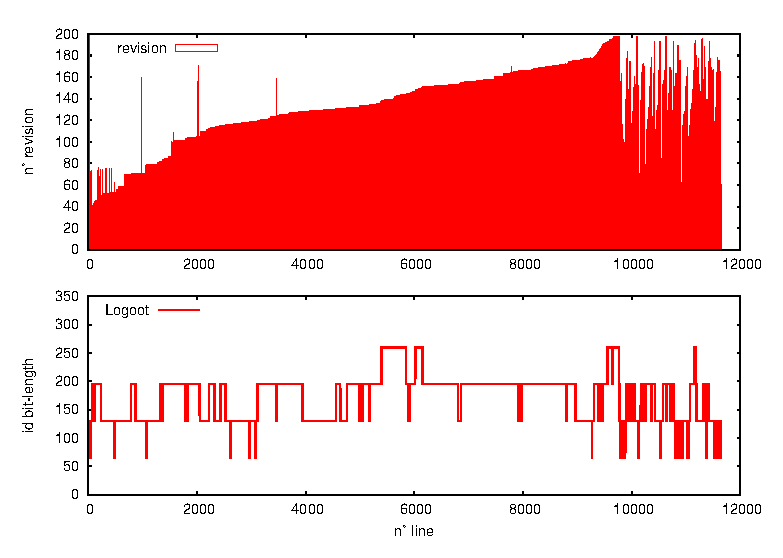
\includegraphics[width=0.48\textwidth]{./img/lseq/compliant.eps}}
  \hspace{10pt}
  \subfloat[Comportement d'édition inattendu]
  [\label{fig:lseq:motivating}Le comportement d'édition va à l'encontre des attentes
  de la stratégie d'allocation]
  {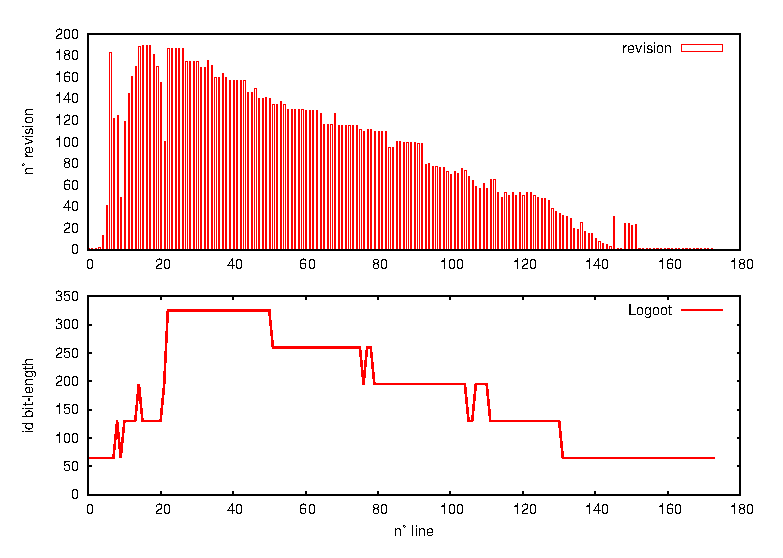
\includegraphics[width=0.48\textwidth]{./img/lseq/motivating.eps}}
  \caption{\label{fig:lseq:allocation}Spectre de documents Wikipedia sous différent
    comportements d'édition antagonistes. La figure du haut représente la
    révision à laquelle la ligne a été insérée, i.e., sa date de naissance.  La
    figure du bas représente la taille de l'identifiant associé à chaque ligne.}
\end{figure*}

Les figures~\ref{fig:lseq:compliant} et~\ref{fig:lseq:motivating} montrent deux
comportements d'éditions présent sur des pages extraites de Wikipedia. La partie
supérieure de ces figures donne une vue globale du comportement d'édition sur la
page. Elle indique la numéro de la révision à laquelle une ligne a été
insérée. Ainsi, plus une barre est haute, plus la ligne a été insérée
récemment. Le spectre de la figure~\ref{fig:lseq:compliant} montre que les
nouveaux éléments de la séquence sont principalement ajoutés en fin. À l'opposé,
le spectre de la figure~\ref{fig:lseq:motivating} montre que les nouveaux
éléments de la séquence sont principalement ajoutés en tête. La partie
inférieure de ces figures montre la taille de la représentation binaire de
l'identifiant associé à chaque élément du document. \TODO{Présenter la stratégie
  d'allocation}. Ainsi, nous observons que les identifiants dans le document
comportant 12k lignes mais principalement édité en fin a des identifiants
n'excédant pas 256 bits. En revanche, le document possédant seulement 170 lignes
édité en tête a des identifiants atteignant déjà les 320 bits.

\TODO{Définition du problème}

%%% Local Variables:
%%% mode: latex
%%% TeX-master: "../../paper"
%%% End:
